\documentclass[a4paper,onecolumn,10pt]{article}
\usepackage[polish]{babel}
\usepackage[utf8]{inputenc}
\usepackage[T1]{fontenc}
\usepackage[left=2.1cm,right=2.1cm]{geometry}
\usepackage[dvipsnames]{xcolor}
\usepackage{amsmath,calc,indentfirst,fancyhdr,amsfonts,graphicx,epstopdf,caption, mathcomp, subcaption,wrapfig, siunitx,pbox,float,algorithm}
\usepackage[noend]{algpseudocode}


\makeatletter
\def\BState{\State\hskip-\ALG@thistlm}
\renewcommand{\ALG@name}{Algorytm}
\makeatother

\renewcommand{\baselinestretch}{1.1}	 % odstep miedzy liniami
\addto\captionspolish{\renewcommand{\figurename}{Wykres}} % zmiana podpisu pod obrazkami, zamiast "Rysunek" bedzie "Wykres"
\newcommand{\NN}{\mathbb{N}}			 % makro do znaku liczb naturalnych

\newcommand{\R}[1]{\textcolor{red}{#1}}  % makro do polecenia z parametrami - tutaj 1 parametr
\newcommand{\G}[1]{\textcolor{green}{#1}} 
\newcommand{\B}[1]{\textcolor{RoyalBlue}{#1}} 
% kolorowanie {\B{argument}}

\newcommand{\PICTURES}{} % szybsza kompilacja dzieki stalej "usuwajacej" obrazki
						 % zakomentowanie \PICTURES powoduje znikniecie obrazkow

\pagestyle{fancy} % formatuj caly dokument
\fancyhead{}
\fancyfoot{}
\renewcommand{\headrulewidth}{0pt}
\fancyfoot[R]{\thepage} % dla stron poza tytulowa nr w prawym dolnym rogu

\fancypagestyle{plain}{ % dla strony tytulowej nr w prawym dolnym rogu
	
	\renewcommand{\headrulewidth}{0pt}
	\fancyhf{}
	\fancyfoot[R]{\thepage}
}

\title{\Large\vspace{-2.5cm}{\Huge S}PRAWOZDANIE - LABORATORIUM NR {\Huge3}\\
		\textbf{Metoda największego spadku \\dla macierzy wstęgowej} } 
\date{\Large14 marca 2019}
\author{\Large Marek Kiełtyka}

\begin{document}
\maketitle

\section{Wstęp}
	
\subsection{Metoda największego spadku}

Jako jedna z iteracyjnych metod rozwiązywania układów równań liniowych postaci
\begin{equation}
[A][x] = [b] 
\label{macierze}
\end{equation} (gdzie \textbf{A} - macierz wejściowa, \textbf{b} - wektor wyrazów wolnych), polega ona na estymowaniu coraz bardziej dokładnego wektora rozwiązań $ x $ na podstawie obliczeń w poprzednich iteracjach. Na potrzeby algorytmu wprowadza się wektor reszt $ r $ będący różnicą między obiema stronami równania (\ref{macierze}). 

\subsection{Pseudokod}

Poczynając od inicjalizacji $b \text{ oraz } x$, poprzez kolejne przybliżenia wyniku dąży się do osiągnięcia zadanego progu zbieżności przez wektor reszt. Jeśli ten próg zostanie osiągnięty, problem można uznać za rozwiązany. Poniższe instrukcje definiują proces postępowania.
\begin{alignat*}{3}
	do \text{ \{ } r_k &= b - Ax_k \\
	\alpha_k &= \frac{r^T_k \cdot r_k}{r^T_k \cdot Ar_k} \\
	x_{k+1} &= x_k + \alpha_kr_k \\
\text{ \} } &while (||r_k||_2 > 10^{-6}) 
\end{alignat*}

Zmienna $k$ oznacza tutaj numer iteracji, wartości $ r_k, \alpha_k, x_k $ są pamiętane tylko podczas danego obiegu pętli. Dla pojedynczej precyzji próg zbieżności założono na poziomie $ 10^{-3} $, dla podwójnej - jak w powyższym pseudokodzie. Transpozycje wektorów nie są konieczne w czasie wykonania programu z uwagi na jednoznaczność reprezentacji w pamięci komputera.

\section{Zadanie do wykonania}

\subsection{Opis problemu}

Celem laboratorium było rozwiązanie układu równań liniowych postaci (\ref{macierze}) przy użyciu opisywanej metody i przedstawienie go na wykresie. Założono następujące warunki początkowe:
\begin{alignat*}{4}
a_{i,j} &= \frac{1}{1 + |i - j|}\text{, } &|i - j| \leq 5 \text{ dla }i,j = 1, \dots , n \\
a_{i,j} &= 0\text{, }  &|i - j| > 5 \text{ dla }i,j = 1, \dots , n 
\end{alignat*}
\begin{alignat*}{4}
N &= 1000 &\text{ - rozmiar macierzy } A \\
b_i &= i &\text{ dla }i = 1, \dots , n \\
x_{i1} &= 0 &\text{ dla }i = 1, \dots , n \\
x_{i2} &= 1 &\text{ dla }i = 1, \dots , n 
\end{alignat*}
Należało zaimplementować algorytm i wykorzystać go osobno dla wektorów $ x_{i1}, x_{i2} $. Ważne było wykonanie pomiaru czasu obliczeń i porównanie go z czasem odpowiadającym metodzie Gaussa-Jordana dla analogicznego problemu.
\subsection{Wyniki}
Do opracowania rozwiązania użyto bibliotek: \textit{Numerical Recipes} i opracowanej samodzielnie, która bazuje na wspomnianej bibliotece \textit{NR} i znacząco ułatwia zapis operacji algebraicznych. W każdej iteracji wyznaczano wartości norm euklidesowych wektorów reszt i rozwiązań.

\begin{equation}
\begin{cases}
||r_k||_2 = \sqrt{r_{k}^{T}r_k} \\
||x_k||_2 = \sqrt{x_{k}^{T}x_k}
\end{cases}
\end{equation}

W sumie rozwiązano pięć układów równań - po dwa dla pojedynczej i podwójnej precyzji $ ( \vec{x}_{1} = 0 \text{ oraz } \vec{x}_{2} = 1 ) $, a także jeden metodą eliminacji zupełnej. Pomiary czasu wykonano tylko dla typu \textit{float}.

\begin{figure}[h!]
	\begin{center}
		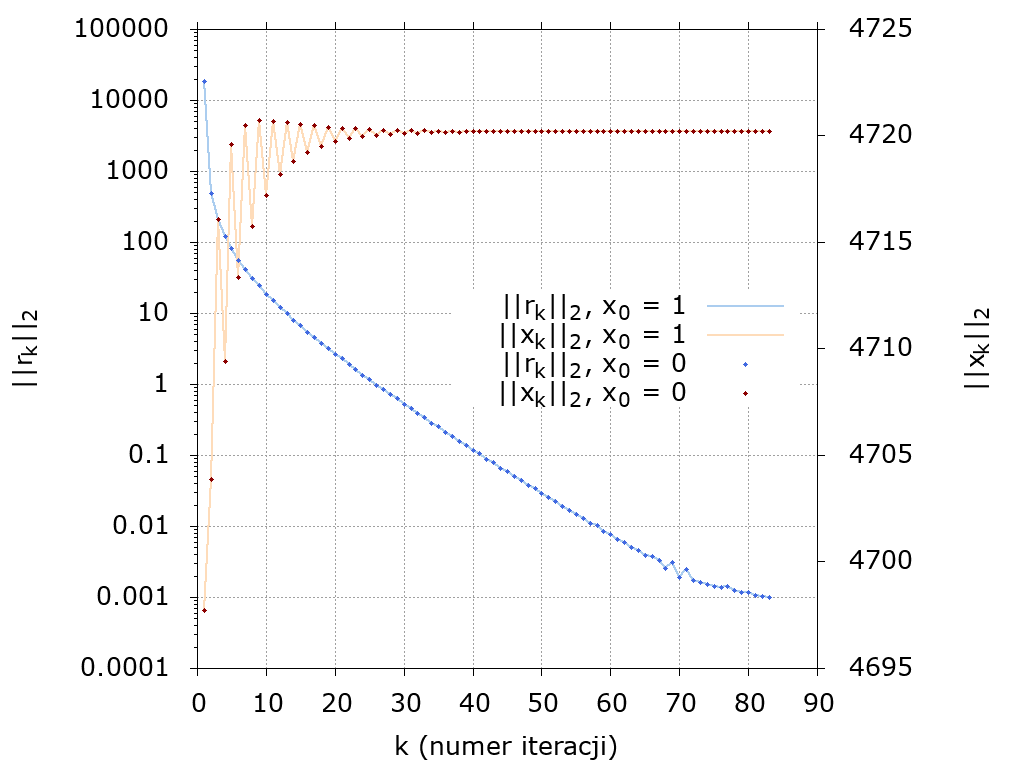
\includegraphics[height=0.6\linewidth]{float.png}
		\caption{Norma wektora reszt $ ||r_k||_2 $ oraz norma wektora rozwiązań $ ||x_k||_2 $ w funkcji numeru iteracji dla pojedynczej precyzji i zbieżności $ 10^{-3} $.}
		\label{float}
	\end{center}
\end{figure}

\begin{table}[!hb]
	\centering
	\begin{tabular}{|c|c|c|}
		\hline
		Lp. & Największego spadku ( $N = 1000$ )& Eliminacji zupełnej ( $N = 400$ )  \\ \hline
		1&719.163 & 758.858 \\ \hline
		2&710.449 & 757.143 \\ \hline
		3&703.752 & 754.007 \\ \hline
		4&708.115 & 763.167 \\ \hline
		5&703.155 & 757.843 \\ \hline
		6&701.794 & 752.966 \\ \hline
		7&702.043 & 754.356 \\ \hline
		8&703.772 & 754.839 \\ \hline
		9&699.344 & 753.149 \\ \hline
		10&704.403 & 751.317 \\ \hline
	\end{tabular}
	\caption{Porównanie czasów rozwiązania dla obu metod i różnych rozmiarów macierzy w milisekundach. Pojedyncza precyzja.}
	\label{tabela}
\end{table}

\newpage
\begin{figure}[h!]
	\begin{center}
		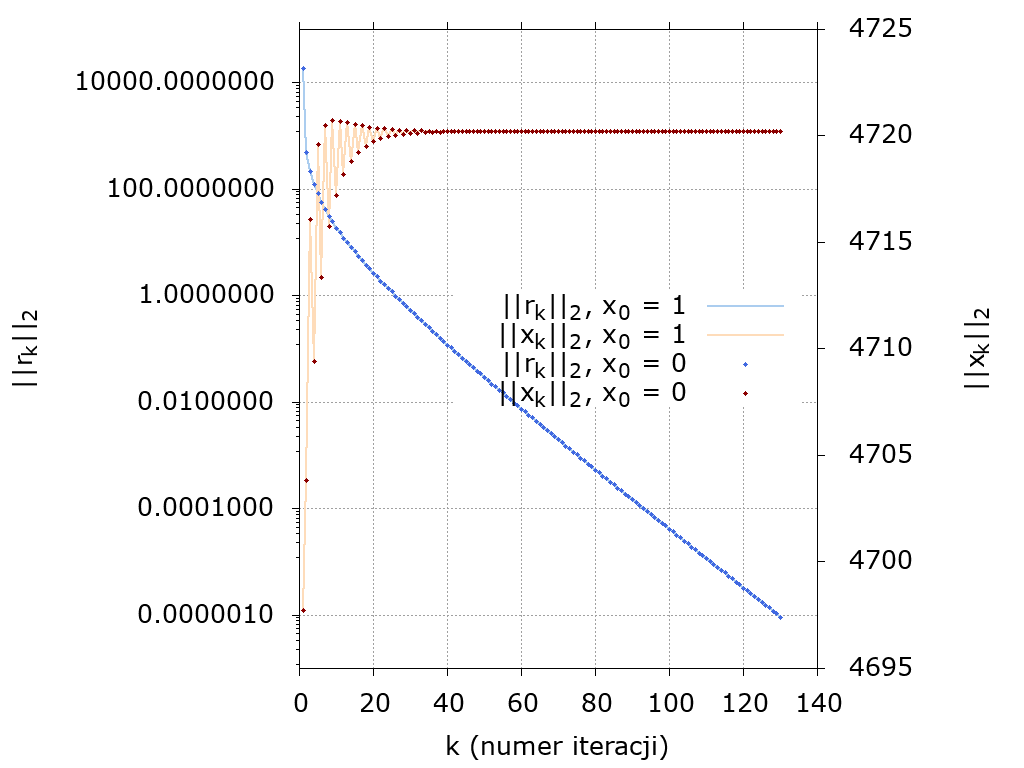
\includegraphics[height=0.6\linewidth]{double.png}
		\caption{Norma wektora reszt $ ||r_k||_2 $ oraz norma wektora rozwiązań $ ||x_k||_2 $ w funkcji numeru iteracji dla podwójnej precyzji i zbieżności $ 10^{-6} $.}
	\end{center}
	\label{double}
\end{figure}
\section{Wnioski}

Patrząc na wykresy można stwierdzić, że początkowe wartości elementów wektora $ \vec{x} $ nie wpływają w żaden sposób na rozwiązanie - widać idealne pokrycie obu przypadków. Mimo założenia tak niskich progów zbieżności, norma wektora $ \vec{x} $ stabilizuje się w okolicach czterdziestej iteracji, co pokazuje szybkość metody największego spadku.

Kolejnym dowodem na efektywność jest zawartość tablicy (\ref{tabela}). Macierz wejściowa może składać się nawet z miliona elementów, a mimo to uzyskujemy rozwiązanie szybciej niż choćby dla $ 160 $ $ 000 $ elementów w przypadku klasycznej metody Gaussa-Jordana. Różnica bierze się również z tego, że do mnożenia macierzy przez wektor użyto ulepszonego algorytmu z uwagi na rzadkość macierzy wejściowej. Celowo nie umieściłem w\,tabeli wyniku metody eliminacji zupełnej dla $ N = 1000 $ przez rosnący wykładniczo czas oczekiwania na rezultaty.

Rozwiązując problem, możnaby również dokonać optymalizacji pamięciowej, gdyż nonsensem jest pamiętanie licznych zerowych elementów tak dużej macierzy, które nic nie wnoszą do wyniku. Wystarczy przechowywać w pamięci tylko główną przekątną oraz znaczące przekątne znajdujące się nad oraz pod główną diagonalą, co znacząco oszczędziłoby niezbędne zasoby pamięci.



\end{document}